\begin{frame}
	\frametitle{Constraint Programming}
	Also called \textit{Combinatorial Optimization}.

	\vspace{1cm}

	A programming paradigm where you are describing the charactersitics of a solution
	rather than the steps needed to reach a solution.
\end{frame}

\begin{frame}
	\frametitle{Solving a Problem in 3 easy steps!}

	\begin{enumerate}
		\item Identifying variables and corresponding domains
		\item Determining Constraints
		\item Choosing a search heuristic
	\end{enumerate}
\end{frame}

\begin{frame}
	\frametitle{Identifying Variables}
	$SEND + MOST = MONEY$
	
	\vspace{0.5cm}
	\noindent
	$S \in \{0, 1, 2, 3, 4, 5, 6, 7, 8, 9\}$ \\
	$E \in \{0, 1, 2, 3, 4, 5, 6, 7, 8, 9\}$ \\
	$N \in \{0, 1, 2, 3, 4, 5, 6, 7, 8, 9\}$ \\
	$D \in \{0, 1, 2, 3, 4, 5, 6, 7, 8, 9\}$ \\
	$M \in \{0, 1, 2, 3, 4, 5, 6, 7, 8, 9\}$ \\
	$O \in \{0, 1, 2, 3, 4, 5, 6, 7, 8, 9\}$ \\
	$T \in \{0, 1, 2, 3, 4, 5, 6, 7, 8, 9\}$ \\
	$Y \in \{0, 1, 2, 3, 4, 5, 6, 7, 8, 9\}$
\end{frame}

\begin{frame}
	\frametitle{Determining Constraints}
	Relationship between variables.

	\begin{tabular}{cccccc}
		& & $1000 * S$ & $100 * E$ & $10 * N$ & $D$ \\
		+ &	& $1000 * M$ & $100 * O$ & $10 * S$ & $T$ \\
		\hline
		& $10000 * M$ & $1000 * O$ & $100 * N$ & $10 * E$ & $Y$
	\end{tabular}

\end{frame}

\begin{frame}
	\frametitle{Choosing a Search Heuristic}
	Search heuristic is a fancy word for "how we want to guess".
	
	\vspace{1cm}

	When we can no longer shrink domains but there are still multiple possibilities we guess.
\end{frame}

\begin{frame}
	\frametitle{Propagating and Searching}
	\begin{columns}
		\begin{column}{0.5\textwidth}
			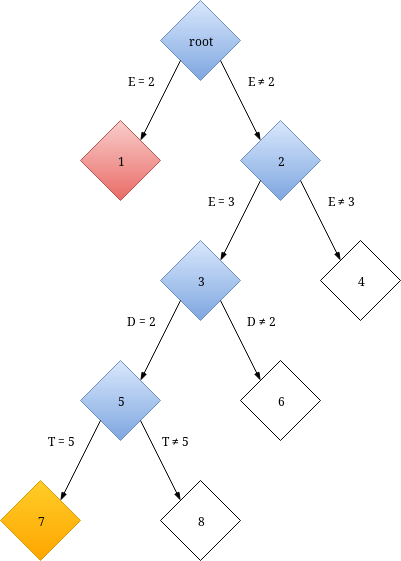
\includegraphics[width=6cm]{../background/constraint-programming/figures/constraint_first_solution}
		\end{column}

		\tabcolsep=0.11cm
		\begin{column}{0.5\textwidth}
			\begin{tabular}{c|c|c|c|c|c}
				Variable & root & 2 & 3 & 5 & 7 \\
				\hline
				S & 9 & 9 & 9 & 9 & 9 \\
				E & 2..7 & 3..7 & 3 & 3 & 3 \\
				N & 3..8 & 4..8 & 4 & 4 & 4 \\
				D & 2..8 & 2..8 & 2,5,6 & 2 & 2 \\
				M & 1 & 1 & 1 & 1 & 1 \\
				O & 0 & 0 & 0 & 0 & 0 \\
				T & 2..8 & 2..8 & 2,5,6 & 5,6 & 5 \\
				Y & 2..8 & 2..8 & 5..8 & 7,8 & 7 \\
			\end{tabular}

		\end{column}
	\end{columns}
\end{frame}

\begin{frame}
	\frametitle{Optimizing}
	Unexplored options

	\vspace{1cm}

	For further combinations to be considered a solution we require $MONEY$ to map to a bigger integer.

	\vspace{1cm}
	
	\centering
	\begin{tabular}{c|c|c|c|c|c|c|c|c}
		S & E & N & D & M & O & T & Y & MONEY \\
		\hline
		9 & 7 & 8 & 2 & 1 & 0 & 4 & 6 & 10876 \\
	\end{tabular}

\end{frame}
